\documentclass[a4paper]{article}

\usepackage[swedish]{babel}
\usepackage[utf8x]{inputenc}
\usepackage{amsmath}
\usepackage{amssymb}
\usepackage[T1]{fontenc}
\usepackage{graphicx}
\usepackage{epstopdf}

\title{Komplettering}

\begin{document}

\maketitle

\section*{2.2}

Här användes \textsc{Matlab} för att illustrera delsummorna till

\begin{align}
  \frac{3\pi}{4} + \sum_{k=1}^{+\infty}\frac{(-1)^k-1}{\pi k^2}\cos (kt) + \frac{1}{k}\sin (kt).\label{eq:22fourier}
\end{align}

se Figur \ref{fig:serie22}

\begin{figure}[h!]
  \centering
  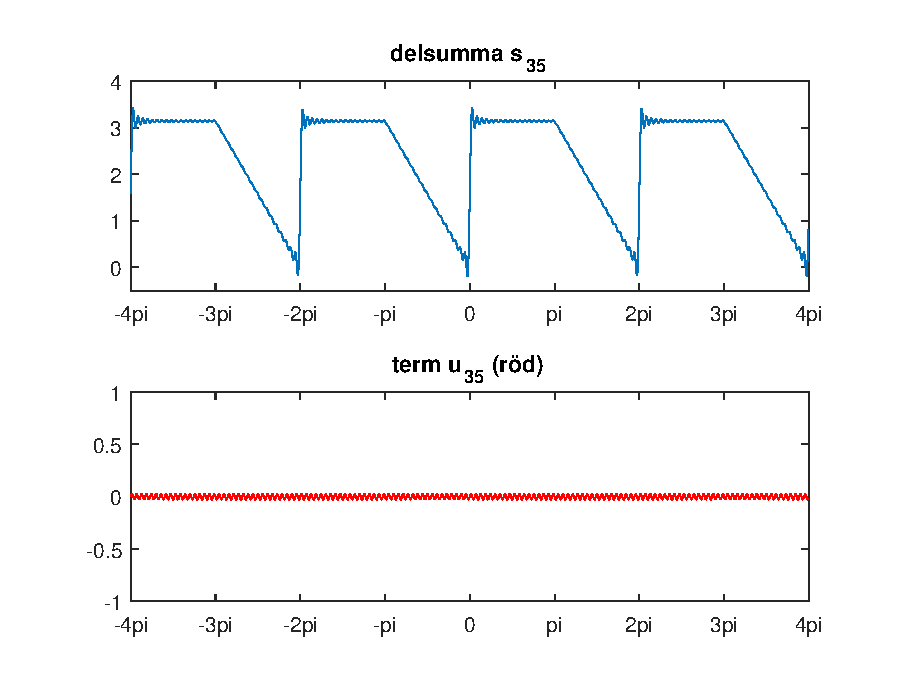
\includegraphics[width=0.75\linewidth]{serie22.eps}
  \caption{}
  \label{fig:serie22}
\end{figure} 

\noindent Härefter gjordes gissningen att (\ref{eq:22fourier}) utvecklas till funktionen

\begin{align*}
  f(t) =
  \begin{cases}
    \pi, 0 \leq t < \pi,\\
    -t + 2\pi, \pi \leq t \leq 2\pi
  \end{cases}.
\end{align*}

För att bekräfta detta tas Fourierkoefficienterna fram ur definitionen av
den trigonometriska Fourierserien för $f(t)$, d.v.s.

\begin{align*}
  \mathcal{FS}_f^{\text{trig}} = \frac{3\pi}{4} + \sum_{k=1}^{+\infty}\left( a_k\cos(k\Omega t) + b_k\sin(k\Omega t) \right)
\end{align*}

\noindent där perioden $T = 2\pi$ fås ur figuren, och $\Omega =
\frac{2\pi}{2\pi} = 1$. Ur definitionen av Fourierkoefficienterna fås då

\setlength{\jot}{10pt}
\begin{align*}
  a_k &= \frac{2}{T}\int_{\text{p}}f(t)\cos(k\Omega t) dt = \frac{1}{\pi}\int_0^{2\pi}f(t)\cos(kt)dt\\
      &= \frac{1}{\pi}\int_0^{\pi}f(t)\cos(kt)dt + \frac{1}{\pi}\int_{\pi}^{2\pi}f(t)\cos(kt)dt\\
      &= \frac{1}{\pi}\int_0^{\pi}\pi\cos(kt)dt + \frac{1}{\pi}\int_{\pi}^{2\pi}(-t + 2\pi)\cos(kt)dt\\
      & = \left[ \frac{\sin(kt)}{k} \right]_0^{\pi} + \frac{1}{\pi}\left( \left[ (-t + 2\pi)\frac{\sin(kt)}{k} \right]_{\pi}^{2\pi} - \int_{\pi}^{2\pi}\frac{\text{d}}{\text{dt}}(-t + 2\pi)\frac{\sin(kt)}{k}dt \right)\\
      &= 0 + \frac{1}{\pi}\left( 0 + \int_{\pi}^{2\pi}\frac{\sin(kt)}{k}dt \right) = \frac{1}{\pi}\left[ -\frac{\cos(kt)}{k^2} \right]_{_pi}^{2\pi}\\
  &= \frac{1}{\pi}\left( \frac{1}{k^2}(-\cos(2\pi k) + cos(\pi k)) \right) = \frac{(-1)^k - 1}{\pi k^2},
\end{align*}

\noindent där den sista likheten utnyttjar att $\cos(\pi k) = (-1)^k$ om $k \in
\mathbb{Z}_+$. På liknande vis fås koefficienten $b_k$

\begin{align*}
  b_k &= \frac{2}{T}\int_{\text{p}}f(t)\sin(k\Omega t)dt = \frac{1}{\pi}\int_0^{\pi}\pi\sin(kt)dt + \frac{1}{\pi}\int_{\pi}^{2\pi}(-t + 2\pi)\sin(kt)dt\\
      &= \left[ -\frac{\cos(kt)}{k} \right]_0^{\pi} + \frac{1}{\pi}\left( \left[ (-t+2\pi)\frac{-\cos(kt)}{k} \right]_{\pi}^{2\pi} + \int_{\pi}^{2\pi}-\frac{\cos(kt)}{k}dt \right)\\
      &= -\frac{\cos(\pi k)}{k} + \frac{1}{k} + \frac{1}{\pi}\left( \left( 0 + \pi\frac{\cos(\pi k)}{k} \right) - \left[ \frac{\sin(kt)}{k^2} \right]_{\pi}^{2\pi} \right)\\
  &= \frac{1}{k}.
\end{align*}

\noindent Koefficienten för $k = 0$ kan inte beräknas ur formlerna för $a_k$
eller $b_k$ då båda dividerar med $k$, istället fås $c_0$ enligt

\begin{align*}
  c_0 &= \frac{a_0}{2} = \frac 12 \cdot \frac 2T \int_{\text{p}}f(t)\cos(k\Omega t)dt\\
  &= \frac 1T \int_0^{2\pi}f(t)dt = \frac 1T \left( \int_0^{\pi}\pi dt + \int_\pi^{2\pi}(-2 + 2\pi) dt \right)\\
  &= \frac 1T \left( \pi^2 + \frac{\pi^2}{2} \right) = \frac{3\pi}{4}.
\end{align*}

Koefficienterna $a_k$, $b_k$ och $c_0$ överensstämmer med de i ekvataion
(\ref{eq:22fourier}), så gissningen av $f(t)$ måste överensstämma med funktionen
som serieutvecklas.

\section*{2.4}

Enligt uppgiften definieras dilogaritmen som

\begin{align*}
  \text{Li}_2 = \sum_{k=1}^{+\infty}\frac{z^k}{k^2}.
\end{align*}

\subsection*{a)}

För vilka värden konvergerar dilogaritmen?

Kvotestet ger här

\begin{align*}
  \kappa = \lim_{k\to\infty}\frac{\left|\frac{z^{k+1}}{(k+1)^2}\right|}{\left|\frac{z^k}{k^2}\right|} = \lim_{k\to\infty}\left| \frac{z^{k+1}k^2}{z^k(k+1)^2}\right| = |z|\lim_{k\to\infty}\frac{k^2}{(k+1)^2} = |z|.
\end{align*}

\noindent Dilogaritmen konvergerar för alla $z$ som uppfyller $\kappa < 1$, d.v.s. då $|z|
< 1$, men notera även att om $|z| = 1$ så fås p-serien med $p = 2$, vilket är en
känd konvergent serie (kvottestet ger ingen info då $\kappa = 1$, d.v.s. då $|z|
= 1$). Sammanfattningsvis så konvergerar serien på enhetscirkeln (inklusive randen).

\section*{Maple}

\emph{(se appendix för första inlämningen för själva Maplekörningen.)}

Jämförelse av Maples resultat och beräkningarna som gjordes för hand i uppgfit
1, visar att Maple ger fel resultat i deluppgift g), samt att programmet inte
känner igen att serierna i deluppgift e) och f) är divergenta. Anledningen till
detta är att Maple inte kan ge ett närmevärde eller ens få fram en formel för en
divergent serie.

I fallet med deluppgift g) så ger Maple ett vilseledande
resultat. Serien är divergent, men Maple ger $-0.7854\ldots$. Exakt vad detta
beror på är oklart, det kan ha något att göra med att serien i g) är divergent
och alternerande. Samma beteende uppvisas om den divergenta, alternerade serien
$\sum_1^{\infty}(-1)^k$ försöker beräknas.

Det är även värt att notera Maples resultat för deluppgift b). Serien är
konvergent och Maple ger ett resultat som tyder på det, men resultatet
innehåller en funktion $\Psi(z_1, z_2)$ som aldrig definieras. En titt i Maples
dokumentation visar följande

\begin{quote}
  Rational functions of k are summed using the algorithm that solves the additive decomposition problem of rational functions. The result is a rational function plus a sum of terms involving the Polygamma function and its derivatives.
\end{quote}

\noindent Funktionen $\Psi$ är därmed polygamma-funktionen, men exakt vad detta
säger om själva serien är oklart.

\end{document}
